\chapter[PROJETO E IMPLEMENTAÇÃO DO SERVIÇO DE PROCESSAMENTO]{PROJETO E IMPLEMENTAÇÃO DO SERVIÇO DE PROCESSAMENTO}

\label{chapter:architecture}

Escolhemos a \textbf{Arquitetura Kappa} como padrão de projeto para servir
de base para o novo serviço de processamento de dados do InterSCity.
A Arquitetura Lambda não justifica a maior complexidade no contexto atual da
plataforma, de modo que essa escolha facilita a manutenibilidade e adoção do
serviço pelo time atual do InterSCity. A Arquitetura Kappa permitirá a análise
em tempo-real sem que ocorra perda de informações relevantes, o que é
importante no contexto de cidades inteligentes, ao passo em que permite a
análise de dados históricos, desde que tenha ocorrido o pré-processamento.
Essa decisão resultou na necessidade de escolha de uma tecnologia de
processamento \textit{streaming} e de um \textit{broker} adequado.

Escolhemos o \textbf{Apache Spark} como tecnologia de \textit{streaming}
a ser usada, por dispor nativamente de biblioteca de clusterização
e aprendizagem de máquina. O Spark ainda facilita, caso necessário, a
troca para a Arquitetura Lambda, por dispor de processamento \textit{batch}.
Escolhemos o \textbf{Apache Kafka} como o \textit{broker} do novo serviço de
processamento, sendo essa uma escolha menos óbvia que a anterior. Embora o
RabbitMQ já seja utilizado pelo InterSCity e tenha vantagens em certos aspectos
em relação ao Kafka, tomamos essa decisão pelo RabbitMQ não dispor de uma
interface nativa que o conecte ao Spark. Outro fator que levamos em conta é o
fato do Kafka ter gerenciamento nativo de \textit{log}, que ajuda na
implantação da Arquitetura Kappa. Contudo, só utilizamos o Kafka no serviço
de processamento de dados, não forçando mudanças no ecossistema de
microsserviços do InterSCity. A Figura \ref{fig:stack} ilustra a pilha de
tecnologias que deve compor a Arquitetura Kappa no InterSCity e as principais
relações entre os diferentes serviços.

\begin{figure}
  \centering
    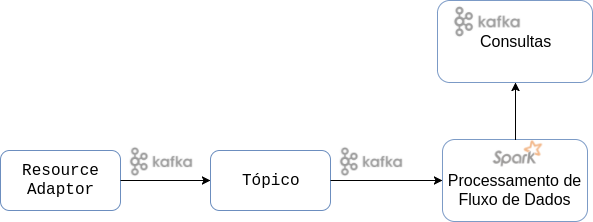
\includegraphics[scale=0.5]{figuras/kappa_tools2.png}
  \caption{Pilha de tecnologias utilizadas - Apache Kafka e Apache Spark, e suas
    interações com o InterSCity.}
  \label{fig:stack}
\end{figure}

\section{IMPLEMENTAÇÃO}

Dividimos a implementação da Arquitetura Kappa em três etapas:
(i) configuração do ambiente, contemplando as ferramentas escolhidas;
(ii) ligações entre os diferentes serviços, tornando possível a publicação de
    mensagens no Kafka e sendo possível seu processamento no Spark; e
(iii) disponibilização de \textit{hooks} que possam ser estendidos futuramente,
    possibilitando a criação de um \textit{pipeline de dados} customizável.

Durante a implementação do novo serviço de processamento de dados para o
InterSCity desenvolvemos o \textbf{Shock}, responsável por abstrair as
comunicações entre as diferentes
ferramentas e trazer a extensibilidade mencionada na terceira etapa da
implementação. Apresentamos no Apêndice \ref{appendix:impl}
pseudo algoritmos que ilustram o uso das ferramentas escolhidas na
implementação da Arquitetura Lambda\footnote{
Pseudo códigos para a Arquitetura Lambda foram disponibilizados como forma
de complemento, pois o Shock já contempla a Arquitetura Kappa.
}.

\begin{figure}
  \centering
    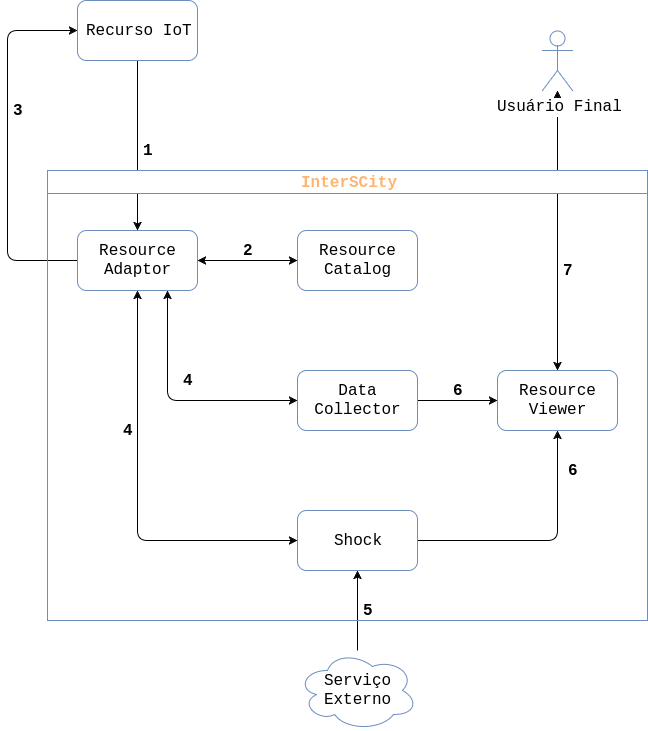
\includegraphics[scale=0.45]{figuras/shock_usage.png}
    \caption{Novo ciclo de vida da plataforma, com relação ao novo serviço de processamento.}
  \label{fig:shock_usage}
\end{figure}

A Figura \ref{fig:shock_usage} ilustra o novo fluxo completo do InterSCity com
a adição do novo serviço de processamento de dados. O início do fluxo (passos 1
ao 3) continua o mesmo, e foi detalhado na Seção \ref{sec:architecture}. As
mudanças começam quando o (4) Resource Adaptor passa a publicar a chegada de
novos dados no Shock através do Kafka, promovendo extensão ao InterSCity.
Aplicações (5) interagem com o Shock via Kafka, construindo o \textit{pipeline}
de um \textit{stream}, definindo as operações a serem executadas.  Por fim, os
resultados do Shock e do Data Collector (6) serão disponibilizados, podendo ser
consumidos por aplicações como o microsserviço Resource Viewer, que (7)
apresenta dados ao usuário final.

Assim como seguido pelo time do InterSCity, utilizamos o Docker na gerência de
configuração do novo serviço. A configuração do Spark que havia sido feita pelo
time do InterSCity na criação do DataProcessor foi reutilizada, e configuramos
um contêiner com o Kafka. Por fim, ligamos os contêineres configurados com o
microsserviço Resource Adaptor, permitindo assim a interação entre o InterSCity
e as ferramentas definidas para uso.

Iniciamos a ligação entre os projetos com uma adaptação no microsserviço
Resource Adaptor, que com a mudança, passou a publicar em um tópico específico
no Kafka a atualização de novos dados. Essa adaptação não trouxe mudanças
significativas no InterSCity, não afetando o fluxo usual da plataforma.
Desenvolvemos o Shock, responsável por receber mensagens em tópicos
específicos do Kafka e passá-los ao Spark Streaming. O Shock gerencia a
execução de \textit{streams} do Spark, permitindo que usuários terceiros
configurem \textit{streams} no Spark sem ter conhecimento da ferramenta.

\section{SHOCK}

O Shock encontra-se disponível em um repositório no
Gitlab\footnote{\url{https://gitlab.com/DGuedes/shock}}, e o novo microsserviço
de processamento de dados pode ser encontrado em um \textit{fork} do serviço
original\footnote{\url{https://gitlab.com/DGuedes/data-processor}}. O Shock
abstrai o uso das diferentes ferramentas e pode ser customizado
por serviços externos que definem e configuram \textit{streams} para serem
executados. O arquitetura do Shock apresenta pontos de estensão, e possui
um \textit{handler} para a Arquitetura Kappa
desenvolvido\footnote{\url{https://gitlab.com/DGuedes/shock/blob/master/shock/handlers.py}},
mas caso seja desejado o uso de outra estratégia, basta implementar um novo
\textit{handler}.

\begin{figure}
  \centering
    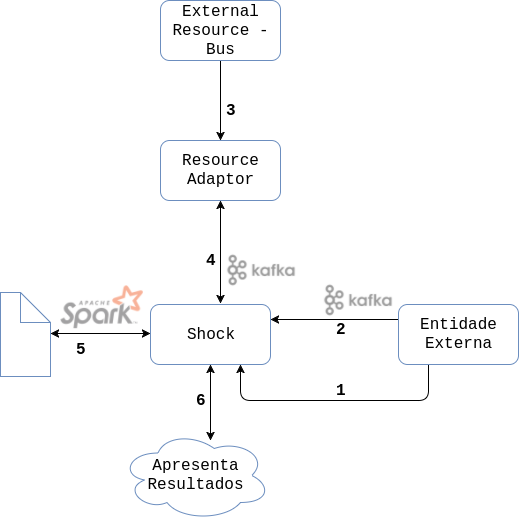
\includegraphics[scale=0.45]{figuras/shock.png}
    \caption{Ciclo de vida do Shock dentro do InterSCity.}
  \label{fig:shock}
\end{figure}

A Figura \ref{fig:shock} ilustra o uso do Shock, utilizando como exemplo uma
aplicação de cidades inteligentes desenvolvida pelo time do
InterSCity\footnote{\url{https://gitlab.com/smart-city-software-platform/external-resources/tree/master/bus}}.
Essa aplicação disponibiliza as coordenadas, o tempo, o índice e a linha de
alguns ônibus de São Paulo. Imaginando que seja desejado a criação de uma nova
informação a partir dos dados dos ônibus, como a \textit{velocidade}, o fluxo
de uso com o Shock poderia ser: (1) um cliente que deseje utilizar o serviço
de processamentos do InterScity analisa as funções que o Shock disponibiliza
para criação do \textit{stream}, e constrói o \textit{stream} desejado através
dessas funções - via Kafka. Os recursos IoT (3) publicam no Resource Adaptor a
chegada de novos dados de ônibus. O Resource Adaptor (4) publica os novos dados
em um tópico específico no Kafka para que sejam recebidos pelo Shock, que os (5)
recebe nos \textit{streams} configurados para ingerir dados naquele tópico, e
os processa através do \textit{pipeline} construído no Passo 2. Por fim, após o
processamento dos dados, o Shock pode (6) disponibilizar os resultados do
processamento, que pode ser reaproveitado por aplicações terceiras.
